\chapter{Boolean Expressions}\label{ch05}
\section{Introduction}

Electronic circuits that do not require any memory devices (like flip-flops or registers) are created using what is called ``Combinational Logic.'' These systems can be quite complex, but all outputs are determined solely by input signals that are processed through a series of logic gates. Combinational circuits can be reduced to a Boolean Algebra expression, though it may be quite complex; and that expression can be simplified using methods developed in this chapter and Chapter \ref{ch06}, \nameref{ch06}, page \pageref{ch06}, and Chapter \ref{ch07}, \nameref{ch07}, page \pageref{ch07}. Combinational circuits are covered in Chapter \ref{ch08}, \nameref{ch08}, page \pageref{ch08}.

In contrast, electronic circuits that require memory devices (like flip-flops or registers) use what is called ``Sequential Logic.'' Those circuits often include feedback loops, so the final output is determined by input signals plus the feedback loops that are processed through a series of logic gates. This makes sequential logic circuits much more complex than combinational and the simplification of those circuits is covered in Chapter \ref{ch09}, \nameref{ch09}, page \pageref{ch09}. 

Finally, most complex circuits include both combinational and sequential sub-circuits. In that case, the various sub-circuits would be independently simplified using appropriate methods. Several examples of these types of circuits are analyzed in Chapter \ref{ch10}, \nameref{ch10}, page \pageref{ch10}.

\section{Creating Boolean Expressions}

A circuit designer is often only given a written (or oral) description of a circuit and then asked to build that device. Too often, the designer may receive notes scribbled on the back of a dinner napkin, along with some verbal description of the desired output, and be expected to build a circuit to accomplish that task. Regardless of the form of the request, the process that the designer follows, in general, is: 

\begin{enumerate}
  \item \textsc{Write The Problem Statement}. The problem to be solved is written in a clear, concise statement. The better this statement is written the easier each of the following steps will be, so time spent polishing the problem statement is worthwhile. 
  
  \item \textsc{Construct A Truth Table}. Once the problem is clearly defined, the circuit designer constructs a truth table where all inputs/outputs are included. It is essential that all possible input combinations that lead to a \emph{True} output are identified. 
  
  \item \textsc{Write A Boolean Expression}. When the truth table is completed, it is easy to create a Boolean expression from that table as covered in Example \ref{05:subsec:example}. 
  
  \item \textsc{Simplify the Boolean Expression}. The expression should be simplified as much as possible, and that process is covered in this chapter, Chapter \ref{ch06}, \nameref{ch06}, page \pageref{ch06}, and Chapter \ref{ch07}, \nameref{ch07}, page \pageref{ch07}. 
  
  \item \textsc{Draw The Logic Diagram}. The logic diagram for a circuit is constructed from the simplified Boolean expression. 
  
  \item \textsc{Build The Circuit}. If desired, a physical circuit can be built using the logic diagram. 
\end{enumerate}

\subsection{Example}
\label{05:subsec:example}

A machine is to be programmed to help pack shipping boxes for the ABC Novelty Company. They are running a promotion so if a customer purchases any two of the following items, but not all three, a free poster will be added to the purchase: joy buzzer, fake blood, itching powder. Design the logic needed to add the poster to appropriate orders. 

\begin{enumerate}
  \item \textsc{Problem Statement}. The problem is already fairly well stated. A circuit is needed that will activate the ``drop poster'' machine when any two of three inputs (joy buzzer, fake blood, itching powder), but not all three, are \emph{True}. 

  \item \textsc{Truth Table}. Let $ J $ be the Joy Buzzer, $ B $ be the Fake Blood, and $ P $ be the Itching Powder; and let the truth table inputs be \emph{True} (or $ 1 $) when any of those items are present in the shipping box. Let the output $ D $ be for ``Drop Poster'' and when it is \emph{True} (or $ 1 $) then a poster will be dropped into the shipping box. The Truth table is illustrated in Table  \ref{05:tab:truth_table_for_example}.
  
  \begin{table}[H]
    \sffamily
    \newcommand{\head}[1]{\textcolor{white}{\textbf{#1}}}    
    \begin{center}
      \rowcolors{2}{gray!10}{white} % Color every other line a light gray
      \begin{tabular}{cccc} 
        \rowcolor{black!75}
        \multicolumn{3}{c}{\head{Inputs}} & \head{Output} \\
        J & B & P & D \\
        \hline
        0 & 0 & 0 & 0 \\
        0 & 0 & 1 & 0 \\
        0 & 1 & 0 & 0 \\
        0 & 1 & 1 & 1 \\
        1 & 0 & 0 & 0 \\
        1 & 0 & 1 & 1 \\
        1 & 1 & 0 & 1 \\
        1 & 1 & 1 & 0
      \end{tabular}
    \end{center}
    \caption{Truth Table for Example}
    \label{05:tab:truth_table_for_example}
  \end{table}
  
  \item \textsc{Write Boolean Expression}. According to the Truth Table, the poster will be dropped into the shipping box in only three cases (when output $ D $ is \emph{True}). Equation \ref{05:eq:example} was generated from the truth table. 
  
  \begin{align}
  \label{05:eq:example}
  BP + JP + JB &= D 
  \end{align}
  
  \item \textsc{Simplify Boolean Expression}. The Boolean expression for this problem is already as simple as possible so no further simplification is needed. 
  
  \item \textsc{Draw Logic Diagram}. Figure \ref{fig:05_01} was drawn from the switching equation.
  
	\begin{figure}[H]
		\centering
		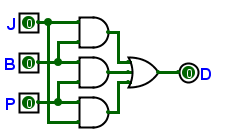
\includegraphics[width=\maxwidth{.95\linewidth}]{gfx/05_01}
		\caption{Logic Diagram From Switching Equation}
		\label{fig:05_01}
	\end{figure}
  
  \item \textsc{Build The Circuit}. This circuit could be built (or ``realized'') with three \textsf{AND}  gates and one 3-input \textsf{OR}  gate. 
  
\end{enumerate}

%***************************************************************************
% Section: Minterms and Maxterms
%***************************************************************************
\section{Minterms and Maxterms}
\label{05:sec:minterms_and_maxterms}

\subsection{Introduction}
\label{05:subsec:introduction_to_minterms_and_maxterms}

The solution to a Boolean equation is normally expressed in one of two formats: \gls{sop} or \gls{pos}.

\subsection{Sum Of Products (SOP) Defined}
\label{05:subsec:sum_of_products_sop_defined}

Equation \ref{05:eq:sop_example} is an example of a \gls{sop} expression. Notice that the expression describes four inputs ($ A $, $ B $, $ C $, $ D $) that are combined through two \textsf{AND} gates and then the output of those \textsf{AND} gates are combined through an \textsf{OR} gate. 

\begin{align}
  \label{05:eq:sop_example}
  (A'BC'D)+(AB'CD) &= Y
\end{align}

Each of the two terms in this expression is a \emph{minterm}. Minterms can be identified in a Boolean expression as a group of inputs joined by an \textsf{AND} gate and then two or more minterms are combined with an \textsf{OR} gate. \marginpar{Notice the inverting bubble on three of the AND gate inputs.}The circuit illustrated in Figure \ref{fig:05_02} would realize Equation \ref{05:eq:sop_example}.

\begin{figure}[H]
	\centering
	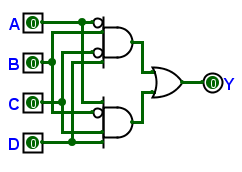
\includegraphics[width=\maxwidth{.95\linewidth}]{gfx/05_02}
	\caption{Logic Diagram For SOP Example}
	\label{fig:05_02}
\end{figure}

\subsection{Product of Sums (POS) Defined}
\label{05:subsec:product_of_sums_pos_defined}

Equation \ref{05:eq:pos_example} is an example of a \gls{pos} expression. Notice that the expression describes four inputs ($ A $, $ B $, $ C $, $ D $) that are combined through two \textsf{OR} gates and then the output of those \textsf{OR} gates are combined through an \textsf{AND} gate. 

\begin{align}
  \label{05:eq:pos_example}
  (A'+B+C+'D)(A+B'+C+D) &= Y
\end{align}

Each term in this expression is called a \emph{maxterm}. Maxterms can be identified in a Boolean expression as a group of inputs joined by an \textsf{OR} gate; and then two or more maxterms are combined with an \textsf{AND} gate. \marginpar{Notice the inverting bubble on three of the OR gate inputs.}The circuit illustrated in Figure \ref{fig:05_03} would realize Equation \ref{05:eq:pos_example}. 

\begin{figure}[H]
	\centering
	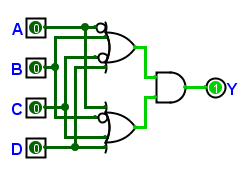
\includegraphics[width=\maxwidth{.95\linewidth}]{gfx/05_03}
	\caption{Logic Diagram For POS Example}
	\label{fig:05_03}
\end{figure}

\subsection{About Minterms}
\label{05:subsec:about_minterms}

A term that contains all of the input variables in one row of a truth table joined with an \textsf{AND} gate is called a minterm. Consider truth table \ref{05:tab:truth_table_for_first_minterm_example} which is for a circuit with three inputs ( $ A $,  $ B $, and  $ C $) and one output ( $ Q $).

\begin{table}[H]
  \sffamily
  \newcommand{\head}[1]{\textcolor{white}{\textbf{#1}}}    
  \begin{center}
    \rowcolors{2}{gray!10}{white} % Color every other line a light gray
    \begin{tabular}{ccc|cc} 
      \rowcolor{black!75}
      \multicolumn{3}{c}{\head{Inputs}} & \multicolumn{2}{c}{\head{Outputs}} \\
      A & B & C & Q & m\\
      \hline
      0 & 0 & 0 & 0 & 0 \\
      0 & 0 & 1 & 0 & 1 \\
      0 & 1 & 0 & 0 & 2 \\
      0 & 1 & 1 & 1 & 3 \\
      1 & 0 & 0 & 0 & 4 \\
      1 & 0 & 1 & 1 & 5 \\
      1 & 1 & 0 & 0 & 6 \\
      1 & 1 & 1 & 0 & 7 
    \end{tabular}
  \end{center}
  \caption{Truth Table for First Minterm Example}
  \label{05:tab:truth_table_for_first_minterm_example}
\end{table}

The circuit that is represented by this truth table would output a \emph{True} in only two cases, when the inputs are $ A'BC $ or $ AB'C $. Equation \ref{05:eq:first_minterm_example} describes this circuit.

\begin{align}
  \label{05:eq:first_minterm_example}
  (A'BC)+(AB'C) &= Q
\end{align}

The terms $ A'BC $ and $ AB'C $ are called \emph{minterms} and they contain every combination of input variables that outputs a \emph{True} when the three inputs are joined by an \textsf{AND} gate. Minterms are most often used to describe circuits that have fewer \emph{True} outputs than \emph{False} (that is, there are fewer $ 1 $'s than $ 0 $'s in the output column). In the example above, there are only two \emph{True} outputs with six \emph{False} outputs, so minterms describe the circuit most efficiently. 

Minterms are frequently abbreviated with a lower-case  $ m $ along with a subscript that indicates the decimal value of the variables. For example, $ A'BC $, the first of the \emph{True} outputs in the truth table above, has a binary value of $ 011 $, which is a decimal value of $ 3 $; thus, the minterm is $ m_3 $. The other minterm in this equation is $ m_5 $ since its binary value is $ 101 $, which equals decimal $ 5 $. It is possible to verbally describe the entire circuit as: $ m_3 $ \textsf{OR} $ m_5 $. For convenience, each of the minterm numbers are indicated in the last column of the truth table.

As another example, consider truth table \ref{05:tab:truth_table_for_second_minterm_example}.

\begin{table}[H]
  \sffamily
  \newcommand{\head}[1]{\textcolor{white}{\textbf{#1}}}    
  \begin{center}
    \rowcolors{2}{gray!10}{white} % Color every other line a light gray
    \begin{tabular}{cccc|cc} 
      \rowcolor{black!75}
      \multicolumn{4}{c}{\head{Inputs}} & \multicolumn{2}{c}{\head{Outputs}} \\
      A & B & C & D & Q & m \\
      \hline
      0 & 0 & 0 & 0 & 1 & 0 \\
      0 & 0 & 0 & 1 & 0 & 1 \\
      0 & 0 & 1 & 0 & 0 & 2 \\
      0 & 0 & 1 & 1 & 0 & 3 \\
      0 & 1 & 0 & 0 & 0 & 4 \\
      0 & 1 & 0 & 1 & 1 & 5 \\
      0 & 1 & 1 & 0 & 1 & 6 \\
      0 & 1 & 1 & 1 & 0 & 7 \\
      1 & 0 & 0 & 0 & 0 & 8 \\
      1 & 0 & 0 & 1 & 0 & 9 \\
      1 & 0 & 1 & 0 & 0 & 10 \\
      1 & 0 & 1 & 1 & 0 & 11 \\
      1 & 1 & 0 & 0 & 0 & 12 \\
      1 & 1 & 0 & 1 & 0 & 13 \\
      1 & 1 & 1 & 0 & 1 & 14 \\
      1 & 1 & 1 & 1 & 0 & 15 
    \end{tabular}
  \end{center}
  \caption{Truth Table for Second Minterm Example}
  \label{05:tab:truth_table_for_second_minterm_example}
\end{table}

Equation \ref{05:eq:second_minterm_example} describes this circuit because these are the rows where the output is \emph{True}.

\begin{align}
  \label{05:eq:second_minterm_example}
  (A'B'C'D')+(A'BC'D)+(A'BCD')+(ABCD') &= Q
\end{align}

These would be minterms $ m_0 $, $ m_5 $, $ m_6 $, and $ m_{14} $. Equation \ref{05:eq:sigma_notation_second_minterm_example} shows a commonly used, more compact way to express this result.

\begin{align}
  \label{05:eq:sigma_notation_second_minterm_example}
  \int(A,B,C,D) &= \sum(0,5,6,14)
\end{align}

Equation \ref{05:eq:sigma_notation_second_minterm_example} would read: ``For the function of inputs  $ A $,  $ B $,  $ C $, and  $ D $, the output is \emph{True} for minterms $ 0 $, $ 5 $, $ 6 $, and $ 14 $ when they are combined with an \textsf{OR}  gate.'' This format is called \emph{Sigma Notation}, and it is easy to derive the full Boolean equation from it by remembering that $ m_0 $ is $ 0000 $, or $ A'B'C'D' $; $ m_5 $ is $ 0101 $, or $ A'BC'D $; $ m_6 $ is $ 0110 $, or $ A'BCD' $; and $ m_{14} $ is $ 1110 $, or $ ABCD' $. Therefore, the Boolean equation can be quickly created from the Sigma Notation. 

A logic equation that is created using minterms is often called the \emph{Sum of Products} (or \emph{SOP}) since each term is composed of inputs \textsf{AND}ed together (``products'') and the terms are then joined by \textsf{OR} gates (``sums'').

\subsection{About Maxterms}
\label{05:subsec:about_maxterms}

A term that contains all of the input variables joined with an \textsf{OR} gate (``added together'') for a \emph{False} output is called a \emph{maxterm}. Consider Truth Table \ref{05:tab:truth_table_for_first_maxterm_example}, which has three inputs ( $ A $,  $ B $, and  $ C $) and one output ( $ Q $): 

\begin{table}[H]
  \sffamily
  \newcommand{\head}[1]{\textcolor{white}{\textbf{#1}}}    
  \begin{center}
    \rowcolors{2}{gray!10}{white} % Color every other line a light gray
    \begin{tabular}{ccc|cc} 
      \rowcolor{black!75}
      \multicolumn{3}{c}{\head{Inputs}} & \multicolumn{2}{c}{\head{Outputs}} \\
      A & B & C & Q & M \\
      \hline
      0 & 0 & 0 & 1 & 0 \\
      0 & 0 & 1 & 1 & 1 \\
      0 & 1 & 0 & 0 & 2 \\
      0 & 1 & 1 & 1 & 3 \\
      1 & 0 & 0 & 1 & 4 \\
      1 & 0 & 1 & 1 & 5 \\
      1 & 1 & 0 & 0 & 6 \\
      1 & 1 & 1 & 1 & 7 
    \end{tabular}
  \end{center}
  \caption{Truth Table for First Maxterm Example}
  \label{05:tab:truth_table_for_first_maxterm_example}
\end{table}

The circuit that is represented by this truth table would output a \emph{False} in only two cases. Since there are fewer \emph{False} outputs than \emph{True}, it is easier to create a Boolean equation that would generate the \emph{False} outputs. Because the equation describes the \emph{False} outputs, each term is built by \emph{complementing} the inputs for each of the \emph{False} output lines. After the output groups are defined, they are joined with an \textsf{AND} gate. Equation \ref{05:eq:first_maxterm_example} is the Boolean equation for Truth Table \ref{05:tab:truth_table_for_first_maxterm_example}.

\begin{align}
  \label{05:eq:first_maxterm_example}
  (A+B'+C)(A'+B'+C) &= Q
\end{align}

The terms $ A+B'+C $ and $ A'+B'+C $ are called $ maxterms $, and they contain the complement of the input variables for each of the \emph{False} output lines. Maxterms are most often used to describe circuits that have fewer \emph{False} outputs than \emph{True}. In Truth Table \ref{05:tab:truth_table_for_first_maxterm_example}, there are only two \emph{False} outputs with six \emph{True} outputs, so maxterms describe the circuit most efficiently.

Maxterms are frequently abbreviated with an upper-case  $ M $ along with a subscript that indicates the decimal value of the complements of the variables. For example, the complement of $ A+B'+C $, the first of the \emph{False} outputs in Truth Table \ref{05:tab:truth_table_for_first_maxterm_example}, is $ 010 $, which is a decimal value of 2; thus, the maxterm would be $ M_2 $. This can be confusing, but remember that the \emph{complements} of the inputs are used to form the expression. Thus, $ A+B'+C $ is $ 010 $, not $ 101 $. The other maxterm in this equation is $ M_6 $ since the binary value of its complement is $ 110 $, which equals decimal 6. It is possible to describe the entire circuit as a the product of two groups of maxterms: $ M_2 $ and $ M_6 $.

As another example, consider Truth Table \ref{05:tab:truth_table_for_second_maxterm_example}.

\begin{table}[H]
  \sffamily
  \newcommand{\head}[1]{\textcolor{white}{\textbf{#1}}}    
  \begin{center}
    \rowcolors{2}{gray!10}{white} % Color every other line a light gray
    \begin{tabular}{cccc|cc} 
      \rowcolor{black!75}
      \multicolumn{4}{c}{\head{Inputs}} & \multicolumn{2}{c}{\head{Outputs}} \\
      A & B & C & D & Q & M \\
      \hline
      0 & 0 & 0 & 0 & 1 & 0 \\
      0 & 0 & 0 & 1 & 1 & 1 \\
      0 & 0 & 1 & 0 & 1 & 2 \\
      0 & 0 & 1 & 1 & 0 & 3 \\
      0 & 1 & 0 & 0 & 1 & 4 \\
      0 & 1 & 0 & 1 & 1 & 5 \\
      0 & 1 & 1 & 0 & 1 & 6 \\
      0 & 1 & 1 & 1 & 1 & 7 \\
      1 & 0 & 0 & 0 & 1 & 8 \\
      1 & 0 & 0 & 1 & 0 & 9 \\
      1 & 0 & 1 & 0 & 1 & 10 \\
      1 & 0 & 1 & 1 & 1 & 11 \\
      1 & 1 & 0 & 0 & 0 & 12 \\
      1 & 1 & 0 & 1 & 1 & 13 \\
      1 & 1 & 1 & 0 & 1 & 14 \\
      1 & 1 & 1 & 1 & 1 & 15 
    \end{tabular}
  \end{center}
  \caption{Truth Table for Second Maxterm Example}
  \label{05:tab:truth_table_for_second_maxterm_example}
\end{table}

Equation \ref{05:eq:second_maxterm_example} describes this circuit.

\begin{align}
  \label{05:eq:second_maxterm_example}
  (A+B+C'+D')(A'+B+C+D')(A'+B'+C+D) &= Q
\end{align}

These would be maxterms $ M_3 $, $ M_9 $, and $ M_{12} $. Equation \ref{05:eq:pi_notation_second_maxterm_example} shows a commonly used, more compact way to express this result.

\begin{align}
  \label{05:eq:pi_notation_second_maxterm_example}
  \int(A,B,C,D) &= \prod(3,9,12)
\end{align}

Equation \ref{05:eq:pi_notation_second_maxterm_example} would read: ``For the function of  $ A $,  $ B $,  $ C $,  $ D $, the output is \emph{False} for maxterms $ 3 $, $ 9 $, and $ 12 $ when they are combined with an \textsf{AND}  gate.'' This format is called \emph{Pi Notation}, and it is easy to derive the Boolean equation from it. Remember that $ M_3 $ is $ 0011 $, or $ A+B+C'+D' $ (the complement of the inputs), $ M_9 $ is $ 1001 $, or $ A'+B+C+D' $, and $ M_{12} $ is $ 1100 $, or $ A'+B'+C+D $. The original equation can be quickly created from the Pi Notation. 

A logic equation that is created using maxterms is often called the \emph{Product of Sums} (or \emph{POS}) since each term is composed of inputs \textsf{OR} ed together (``sums'') and the terms are then joined by \textsf{AND}  gates (``products'').

\subsection{Minterm and Maxterm Relationships}
\label{05:subsec:minterm_and_maxterm_relationships}

The minterms and maxterms of a circuit have three interesting relationships: equivalence, duality, and inverse. To define and understand these terms, consider Truth Table \ref{05:tab:minterm_and_maxterm_relationships_truth_table} for some unspecified ``black box'' circuit: 

\begin{table}[H]
  \sffamily
  \newcommand{\head}[1]{\textcolor{white}{\textbf{#1}}}    
  \begin{center}
    \rowcolors{2}{gray!10}{white} % Color every other line a light gray
    \begin{tabular}{ccc|cc|cc} 
      \rowcolor{black!75}
      \multicolumn{3}{c}{\head{Inputs}} & \multicolumn{2}{c}{\head{Outputs}} & \multicolumn{2}{c}{\head{Terms}} \\
      A & B & C & Q & Q' & minterm & Maxterm \\
      \hline
      0 & 0 & 0 & 0 & 1 & $ A'B'C' $ ($ m_0 $) & $ A+B+C $    ($ M_0 $) \\
      0 & 0 & 1 & 1 & 0 & $ A'B'C $  ($ m_1 $) & $ A+B+C' $   ($ M_1 $) \\
      0 & 1 & 0 & 0 & 1 & $ A'BC' $  ($ m_2 $) & $ A+B'+C $   ($ M_2 $) \\
      0 & 1 & 1 & 0 & 1 & $ A'BC $   ($ m_3 $) & $ A+B'+C' $  ($ M_3 $) \\
      1 & 0 & 0 & 0 & 1 & $ AB'C' $  ($ m_4 $) & $ A'+B+C $   ($ M_4 $) \\
      1 & 0 & 1 & 1 & 0 & $ AB'C $   ($ m_5 $) & $ A'+B+C' $  ($ M_5 $) \\
      1 & 1 & 0 & 0 & 1 & $ ABC' $   ($ m_6 $) & $ A'+B'+C $  ($ M_6 $) \\
      1 & 1 & 1 & 1 & 0 & $ ABC $    ($ m_7 $) & $ A'+B'+C' $ ($ M_7 $) 
    \end{tabular}
  \end{center}
  \caption{Minterm and Maxterm Relationships}
  \label{05:tab:minterm_and_maxterm_relationships_truth_table}
\end{table}

\subsubsection{Equivalence}
\label{05:subsubsec:equivalence}

The minterms and the maxterms for a given circuit are considered equivalent ways to describe that circuit. For example, the circuit described by Truth Table \ref{05:tab:minterm_and_maxterm_relationships_truth_table} could be defined using minterms (Equation \ref{05:eq:sigma_notation_minterm_and_maxterm_equivalence}).

\begin{align}
  \label{05:eq:sigma_notation_minterm_and_maxterm_equivalence}
  \int(A,B,C) &= \sum(1,5,7)
\end{align}

However, that same circuit could also be defined using maxterms (Equation \ref{05:eq:pi_notation_minterm_and_maxterm_equivalence}).

\begin{align}
  \label{05:eq:pi_notation_minterm_and_maxterm_equivalence}
  \int(A,B,C) &= \prod(0,2,3,4,6)
\end{align}

These two functions describe the same circuit and are, consequently, equivalent. The \emph{Sigma Function} includes the terms $ 1 $, $ 5 $, and $ 7 $ while the \emph{Pi Function} includes all other terms in the truth table ($ 0 $, $ 2 $, $ 3 $, $ 4 $, and $ 6 $). To put it a slightly different way, the \emph{Sigma Function} describes the truth table rows where Q = $ 1 $ (minterms) while the \emph{Pi Function} describes the rows in the same truth table where Q =  $ 0 $ (maxterms). Therefore, Equation \ref{05:eq:minterm_and_maxterm_equivalence} can be derived.

\begin{align}
  \label{05:eq:minterm_and_maxterm_equivalence}
  \sum(1,5,7) &\equiv \prod(0,2,3,4,6)
\end{align}

\subsubsection{Duality}
\label{05:subsubsec:duality}

Each row in Truth Table \ref{05:tab:minterm_and_maxterm_relationships_truth_table} describes two terms that are considered duals. For example, minterm $ m_5 $ ($ AB'C $) and maxterm $ M_5 $ ($ A'+B+C' $) are duals. Terms that are duals are complements of each other ($ Q $ vs. $ Q' $) and the input variables are also complements of each other; moreover, the inputs for the three minterms are combined with an \textsf{AND}  while the maxterms are combined with an \textsf{OR}. The output of the circuit described by Truth Table \ref{05:tab:minterm_and_maxterm_relationships_truth_table} could be defined using minterms (Equation \ref{05:eq:q_output_dual}).

\begin{align}
  \label{05:eq:q_output_dual}
  Q &= \sum(1,5,7)
\end{align}

The dual of the circuit would be defined by using the maxterms for the same output rows. However, those rows are the \emph{complement} of the circuit (Equation \ref{05:eq:q_not_output_dual}).

\begin{align}
  \label{05:eq:q_not_output_dual}
  Q' &= \prod(1,5,7)
\end{align}

This leads to the conclusion that the complement of a \textit{Sigma Function} is the \textit{Pi Function} with the same inputs, as in Equation \ref{05:eq:dual} (the overline was used to emphasize the the fact that the \textit{PI Function} is complemented).

\begin{align}
  \label{05:eq:dual}
  \sum(1,5,7) &= \overline{\prod(1,5,7)}
\end{align}


\subsubsection{Inverse}
\label{05:subsubsec:inverse}

The complement of a function yields the opposite output. For example the following functions are inverses because one defines $ Q $ while the other defines $ Q' $ using only minterms of the same circuit (or truth table).

\begin{align}
  \label{05:eq:q_output_inverse}
  Q &= \sum(1,5,7)
\end{align}

\begin{align}
  \label{05:eq:q_not_output_inverse}
  Q' &= \sum(0,2,3,4,6)
\end{align}

\subsubsection{Summary}
\label{05:subsubsec:summary_minterm_and_maxterm_relationships}

These three relationships are summarized in the following table. Imagine a circuit with two or more inputs and an output of  $ Q $. Table \ref{05:tab:minterm_and_maxterm_relationships} summarizes the various relationships in the Truth Table for that circuit.

\begin{table}[H]
  \sffamily
  \begin{center}
    \begin{tabular}{|l|l|} 
      \hline
      Minterms where Q is 1 & Minterms where Q' is 1 \\
      \hline
      Maxterms where Q is 1 & Maxterms where Q' is 1 \\
      \hline
    \end{tabular}
  \end{center}
  \caption{Minterm-Maxterm Relationships}
  \label{05:tab:minterm_and_maxterm_relationships}
\end{table}

The adjacent items in a single column are equivalent (that is,  $ Q $ Minterms are equivalent to  $ Q $ Maxterms), items that are diagonal are duals ( $ Q $ Minterms and  $ Q' $ Maxterms are duals), and items that are adjacent in a single row are inverses ( $ Q $ Minterms and  $ Q' $ Minterms are inverses). 

\subsection{Sum of Products Example}
\label{05:subsubsec:sum_of_products_example}

\subsubsection{Given}
\label{05:subsubsec:given_sop_example}

A ``vote-counter'' machine is designed to turn on a light if any two or more of three inputs are \emph{True}. Create a circuit to realize this machine. 

\subsubsection{Truth Table}
\label{05:subsubsec:truth_table_sop_example}

When realizing a circuit from a verbal description, the best place to start is constructing a truth table. This will make the Boolean expression easy to write and then make the circuit easy to realize. For the ``vote-counter'' problem, start by defining variables for the truth table: Inputs  $ A $,  $ B $,  $ C $ and Output  $ Q $. 

Next, construct the truth table by identifying columns for each of the three input variables and then indicate the output for every possible input condition (Table \ref{05:tab:truth_table_for_sop_example}).

\begin{table}[H]
  \sffamily
  \newcommand{\head}[1]{\textcolor{white}{\textbf{#1}}}    
  \begin{center}
    \rowcolors{2}{gray!10}{white} % Color every other line a light gray
    \begin{tabular}{ccc|cc} 
      \rowcolor{black!75}
      \multicolumn{3}{c}{\head{Inputs}} & \multicolumn{2}{c}{\head{Outputs}} \\
      A & B & C & Q & m\\
      \hline
      0 & 0 & 0 & 0 & 0 \\
      0 & 0 & 1 & 0 & 1 \\
      0 & 1 & 0 & 0 & 2 \\
      0 & 1 & 1 & 1 & 3 \\
      1 & 0 & 0 & 0 & 4 \\
      1 & 0 & 1 & 1 & 5 \\
      1 & 1 & 0 & 1 & 6 \\
      1 & 1 & 1 & 1 & 7 
    \end{tabular}
  \end{center}
  \caption{Truth Table for SOP Example}
  \label{05:tab:truth_table_for_sop_example}
\end{table}

\subsubsection{Boolean Equation}
\label{05:subsubsec:boolean_equation_sop_example}

In a truth table, if there are fewer \emph{True} outputs than \emph{False}, then it is easiest to construct a Sum-of-Products equation. In that case, a Boolean expression can be derived by creating the minterms for all \emph{True} outputs and combining those minterms with \textsf{OR}  gates. Equation \ref{05:eq:sigma_notation_sop_example} is the \emph{Sigma Function} of this circuit.

\begin{align}
  \label{05:eq:sigma_notation_sop_example}
  \int(A,B,C) &= \sum(3,5,6,7)
\end{align}

% Pull Quote - Marginal Note - Sidebar
\marginpar{It may be possible to simplify the Boolean expression, but that process is covered elsewhere in this book.}

At this point, a circuit could be created with four 3-input \textsf{AND}  gates combined into one 4-input \textsf{OR}  gate.

\subsection{Product of Sums Example}
\label{05:subsubsec:product_of_sums_example}

\subsubsection{Given}
\label{05:subsubsec:given_pos_example}

A local supply company is designing a machine to sort packages for shipping. All packages go to the post office \emph{except} packages going to the local ZIP code containing chemicals (they are shipped by courier) and packages going to a distant ZIP code containing only perishables (they are shipped via air freight).

\subsubsection{Truth Table}
\label{05:subsubsec:truth_table_pos_example}

When realizing a circuit from a verbal description, the best place to start is constructing a truth table. This will make the Boolean expression easy to write and then make the circuit easy to realize. For the sorting machine problem, start by defining variables for the truth table: 

\begin{itemize}
  \item Ship via post office (the Output):  $ O $ is \emph{True} if ship by Post Office
  \item Zip Code:  $ Z $ is \emph{True} if the zip code is local
  \item Chemicals:  $ C $ is \emph{True} if the package contains chemicals
  \item Perishable:  $ P $ is \emph{True} if the package contains perishables
\end{itemize}

Next, construct the truth table by identifying columns for each of the three input variables and then indicate the output for every possible input condition (Table \ref{05:tab:truth_table_for_sop_example}).

\begin{table}[H]
  \sffamily
  \newcommand{\head}[1]{\textcolor{white}{\textbf{#1}}}    
  \begin{center}
    \rowcolors{2}{gray!10}{white} % Color every other line a light gray
    \begin{tabular}{ccc|cc} 
      \rowcolor{black!75}
      \multicolumn{3}{c}{\head{Inputs}} & \multicolumn{2}{c}{\head{Outputs}} \\
      Z & C & P & O & M \\
      \hline
      0 & 0 & 0 & 1 & 0 \\
      0 & 0 & 1 & 0 & 1 \\
      0 & 1 & 0 & 1 & 2 \\
      0 & 1 & 1 & 0 & 3 \\
      1 & 0 & 0 & 1 & 4 \\
      1 & 0 & 1 & 1 & 5 \\
      1 & 1 & 0 & 0 & 6 \\
      1 & 1 & 1 & 0 & 7 
    \end{tabular}
  \end{center}
  \caption{Truth Table for POS Example}
  \label{05:tab:truth_table_for_pos_example}
\end{table}

\subsubsection{Boolean Equation}
\label{05:subsubsec:boolean_equation_pos_example}

In the truth table, if there are fewer \emph{False} outputs than \emph{True} then it is easiest to construct a Products-of-Sums equation. In that case, a Boolean expression can be derived by creating the maxterms for all \emph{False} outputs and combining the complement those maxterms with \textsf{AND}  gates. Equation \ref{05:eq:pi_notation_pos_example} is the \emph{Pi Expression} of this circuit.

\begin{align}
  \label{05:eq:pi_notation_pos_example}
  \int(Z,C,P) &= \prod(1,3,6,7)
\end{align}

% Pull Quote - Marginal Note - Sidebar
\marginpar{It may be possible to simplify the Boolean expression, but that process is covered elsewhere in this book.}

At this point, a circuit could be created with four 3-input \textsf{OR}  gates combined into one 4-input \textsf{AND}  gate.

\subsection{Summary}
\label{05:subsubsec:summary_minterms_and_maxterms}

\gls{sop} Boolean expressions may be generated from truth tables quite easily, by determining which rows of the table have an output of \emph{True}, writing one minterm for each of those rows, and then summing all of the minterms. The resulting expression will lend itself well to implementation as a set of \textsf{AND} gates (products) feeding into a single \textsf{OR} gate (sum). 

\gls{pos} Boolean expressions may be generated from truth tables quite easily, by determining which rows of the table have an output of \emph{False}, writing one maxterm for each of those rows, and then multiplying all of the maxterms. The resulting expression will lend itself well to implementation as a set of \textsf{OR} gates (sums) feeding into a single \textsf{AND} gate (product). 

%***************************************************************************
% Section: Canonical Form
%***************************************************************************
\section{Canonical Form}
\label{05:sec:canonical_form}

\subsection{Introduction}
\label{05:subsec:introduction_to_canonical_form}

The word ``canonical'' simply means ``standard'' and it is used throughout mathematics and science to denote some standard form for equations. In digital electronics, Boolean equations are considered to be in canonical form when each of the terms in the equation includes all of the possible inputs and those terms appear in the same order as in the truth table. Using the canonical form is important when simplifying a Boolean equation. For example, imagine the solution to a given problem generated table \ref{05:tab:canonical_example_truth_table}.

\begin{table}[H]
  \sffamily
  \newcommand{\head}[1]{\textcolor{white}{\textbf{#1}}}    
  \begin{center}
    \rowcolors{2}{gray!10}{white} % Color every other line a light gray
    \begin{tabular}{ccc|cc} 
      \rowcolor{black!75}
      \multicolumn{3}{c}{\head{Inputs}} & \multicolumn{2}{c}{\head{Outputs}} \\
      A & B & C & Q & m \\
      \hline
      0 & 0 & 0 & 0 & 0 \\
      0 & 0 & 1 & 1 & 1 \\
      0 & 1 & 0 & 0 & 2 \\
      0 & 1 & 1 & 1 & 3 \\
      1 & 0 & 0 & 0 & 4 \\
      1 & 0 & 1 & 0 & 5 \\
      1 & 1 & 0 & 0 & 6 \\
      1 & 1 & 1 & 1 & 7 
    \end{tabular}
  \end{center}
  \caption{Canonical Example Truth Table}
  \label{05:tab:canonical_example_truth_table}
\end{table}

Minterm equation \ref{05:eq:canonical_example} is derived from the truth table and is presented in canonical form. Notice that each term includes all possible inputs ( $ A $,  $ B $, and  $ C $), and that the terms are in the same order as they appear in the truth table. 

\begin{align}
  \label{05:eq:canonical_example}
  (A'B'C)+(A'BC)+(ABC) &= Q
\end{align}

Frequently, though, a Boolean equation is expressed in standard form, which is not the same as canonical form. Standard form means that some of the terms have been simplified and not all of the inputs will appear in all of the terms. For example, consider Equation \ref{05:eq:standard_form_example}, which is the solution for a 4-input circuit.

\begin{align}
  \label{05:eq:standard_form_example}
  (A'C)+(B'CD) &= Q
\end{align}

This equation is in standard form so the first term, $ A'C $, does not include inputs  $ B $ or  $ D $ and the second term, $ B'CD $, does not include input  $ A $. However, all inputs must be present in every term for an equation to be in canonical form.

Building a truth table for an equation in standard form raises an important question. Consider the truth table for Equation \ref{05:eq:standard_form_example}.

\begin{table}[H]
  \sffamily
  \newcommand{\head}[1]{\textcolor{white}{\textbf{#1}}}    
  \begin{center}
    \rowcolors{2}{gray!10}{white} % Color every other line a light gray
    \begin{tabular}{cccc|cc} 
      \rowcolor{black!75}
      \multicolumn{4}{c}{\head{Inputs}} & \multicolumn{2}{c}{\head{Outputs}} \\
      A & B & C & D & Q & m \\
      \hline
      0 & 0 & 0 & 0 & 0 & 0 \\
      0 & 0 & 0 & 1 & 0 & 1 \\
      0 & 0 & 1 & 0 & 0 & 2 \\
      0 & 0 & 1 & 1 & ? & 3 \\
      0 & 1 & 0 & 0 & 0 & 4 \\
      0 & 1 & 0 & 1 & 0 & 5 \\
      0 & 1 & 1 & 0 & 0 & 6 \\
      0 & 1 & 1 & 1 & 0 & 7 \\
      1 & 0 & 0 & 0 & 0 & 8 \\
      1 & 0 & 0 & 1 & 0 & 9 \\
      1 & 0 & 1 & 0 & 0 & 10 \\
      1 & 0 & 1 & 1 & ? & 11 \\
      1 & 1 & 0 & 0 & 0 & 12 \\
      1 & 1 & 0 & 1 & 0 & 13 \\
      1 & 1 & 1 & 0 & 0 & 14 \\
      1 & 1 & 1 & 1 & 0 & 15 
    \end{tabular}
  \end{center}
  \caption{Truth Table for Standard Form Equation}
  \label{05:tab:truth_table_for_standard_form_equation}
\end{table}

In what row would $ B'CD $, the second term in Equation \ref{05:eq:standard_form_example}, be placed? $ B'CD $ is $ 011 $ (in binary), but since the $ A $ term is missing would it be a $ 0 $ or $ 1 $; in other words, would $ B'CD $ generate an output of $ 1 $ for row $ 0011\;(m_3)$ or $ 1011\;(m_{11})$? (The output for these two rows are marked with a question mark in Table \ref{05:tab:truth_table_for_standard_form_equation}.) In fact, the output for \emph{both} of these rows must be considered \emph{True} in order to ensure that all possible combinations of input are covered. Thus, the final equation for this circuit must include at least these two terms: $ (A'B'CD) + (AB'CD) $. In the same way, the term $ A'C $ means that the output is \emph{True} for $ m_2 $, $ m_3 $, $ m_6 $, and $ m_7 $ since input $ A'C $ is \emph{True} and any minterm that contains those two value is also considered \emph{True}. Thus, the final equation for this circuit must include at least these four terms: $ (A'B'CD') + (A'B'CD) + (A'BCD') + (A'BCD) $.

\subsection{Converting Terms Missing One Variable}
\label{05:subsec:converting_terms_missing_one_variable}

To change a standard Boolean expression that is missing one input term into a canonical Boolean expression, insert both \emph{True} and \emph{False} for the missing term into the original standard expression. As an example, consider the term $ B'CD $. Since term $ A $ is missing, both $ A $ and $ A' $ must be included in the converted canonical expression. Equation \ref{05:eq:canonical_expanding_3-variable_term} proves that $ B'CD $ can be expanded to include both possible values for $ A $ by using the Adjacency Property (page \pageref{BF:subsec:adjacency_property}).

\begin{align}
  \label{05:eq:canonical_expanding_3-variable_term}
  (B'CD) \rightarrow (AB'CD)+(A'B'CD)
\end{align}

A term that is missing one input variable will expand into two terms that include all variables. For example, in a system with four input variables (as above), any standard term with only three variables will expand to a canonical expression containing two groups of four variables. 

Expanding a standard term that is missing one variable can also be done with a truth table. To do that, fill in an output of $ 1 $ for every line where the \emph{True} inputs are found while ignoring all missing variables. As an example, consider Truth Table \ref{05:tab:truth_table_for_standard_form_equation} where the outputs for $ m_3 $ and $ m_11 $ are marked with a question mark. However, the output for both of these lines should be marked as \emph{True} because  $ B'CD $ is \emph{True} (input $ A $ is ignored). Then, those two minterms lead to the Boolean expression $ AB'CD + A'B'CD $.

\subsection{Converting Terms Missing Two Variables}
\label{05:subsec:converting_terms_missing_two_variables}

It is easiest to expand a standard expression that is missing two terms by first inserting one of the missing variables and then inserting the other missing variable in two distinct steps. The process for inserting a single missing variable is found in Section \ref{05:subsec:converting_terms_missing_one_variable}. Consider the term $ A'C $ in a four-variable system. It is missing both the $ B $ and $ D $ variables. To expand that term to its canonical form, start by inserting either of the two missing variables. For example, Equation \ref{05:eq:canonical_expanding_2-variable_term_step_one} illustrates entering $ B $ and $ B' $ into the expression.

\begin{align}
  \label{05:eq:canonical_expanding_2-variable_term_step_one}
  (A'C) &\rightarrow (A'BC)+(A'B'C)
\end{align}

Then, Equation \ref{05:eq:canonical_expanding_2-variable_term_step_two} illustrates inserting $ D $ and $ D' $ into the expression.

\begin{align}
  \label{05:eq:canonical_expanding_2-variable_term_step_two}
  (A'BC) &\rightarrow (A'BCD)+(A'BCD') \\
  \nonumber
  (A'B'C) &\rightarrow (A'B'CD)+(A'B'CD')
\end{align}

In the end, $ A'C $ expands to Equation \ref{05:eq:canonical_expanding_2-variable_term_step_three}:

\begin{align}
  \label{05:eq:canonical_expanding_2-variable_term_step_three}
  (A'C) \rightarrow &(A'BCD) + (A'BCD') \\
  \nonumber
  &+ (A'B'CD) + (A'B'CD')
\end{align}

Thus, in a four-variable system, any standard term with only two variables will expand to a canonical expression with four groups of four variables.

Expanding a standard term that is missing two variables can also be done with a truth table. To do that, fill in an output of $ 1 $ for every line where the \emph{True} inputs are found while ignoring all missing variables. As an example, consider a Table \ref{05:tab:truth_table_for_expression_with_missing_variables}, where $ A'C $ is marked as \emph{True}:

\begin{table}[H]
  \sffamily
  \newcommand{\head}[1]{\textcolor{white}{\textbf{#1}}}    
  \begin{center}
    \rowcolors{2}{gray!10}{white} % Color every other line a light gray
    \begin{tabular}{cccc|cc} 
      \rowcolor{black!75}
      \multicolumn{4}{c}{\head{Inputs}} & \multicolumn{2}{c}{\head{Outputs}} \\
      A & B & C & D & Q & m \\
      \hline
      0 & 0 & 0 & 0 & 0 & 0 \\
      0 & 0 & 0 & 1 & 0 & 1 \\
      0 & 0 & 1 & 0 & 1 & 2 \\
      0 & 0 & 1 & 1 & 1 & 3 \\
      0 & 1 & 0 & 0 & 0 & 4 \\
      0 & 1 & 0 & 1 & 0 & 5 \\
      0 & 1 & 1 & 0 & 1 & 6 \\
      0 & 1 & 1 & 1 & 1 & 7 \\
      1 & 0 & 0 & 0 & 0 & 8 \\
      1 & 0 & 0 & 1 & 0 & 9 \\
      1 & 0 & 1 & 0 & 0 & 10 \\
      1 & 0 & 1 & 1 & 0 & 11 \\
      1 & 1 & 0 & 0 & 0 & 12 \\
      1 & 1 & 0 & 1 & 0 & 13 \\
      1 & 1 & 1 & 0 & 0 & 14 \\
      1 & 1 & 1 & 1 & 0 & 15 
    \end{tabular}
  \end{center}
  \caption{Truth Table for Standard Form Equation}
  \label{05:tab:truth_table_for_expression_with_missing_variables}
\end{table}

Notice that outputs for $ m_2 $, $ m_3 $, $ m_6 $, and $ m_7 $ are \emph{True} because for each of those minterms $ A'C $ is \emph{True} (inputs $ B $ and $ D $ are ignored). Then, those four minterms lead to the Boolean expression $ A'B'CD'+A'B'CD+A'BCD'+A'BCD $.

\subsection{Summary}
\label{05:subsec:summary_of_canonical_forms}

This discussion started with Equation \ref{05:eq:standard_form_example_repeated}, which is in standard form.

\begin{align}
  \label{05:eq:standard_form_example_repeated}
  (A'C)+(B'CD) &= Q
\end{align}

After expanding both terms, Equation \ref{05:eq:canonical_form_summary_equation_not_simplified} is generated.

\begin{align}
  \label{05:eq:canonical_form_summary_equation_not_simplified}
  &(A'BCD)+(A'BCD')+(A'B'CD) \\
  \nonumber
  +&(A'B'CD')+(AB'CD)+(A'B'CD) = Q
\end{align}

Notice, though, that the term $ A'B'CD $ appears two times, so one of those can be eliminated by the Idempotence property (page \pageref{BF:subsec:idempotence}), leaving Equation \ref{05:eq:canonical_form_summary_equation_simplified}.

\begin{align}
  \label{05:eq:canonical_form_summary_equation_simplified}
  &(A'BCD)+(A'BCD') \\
  \nonumber
  +&(A'B'CD')+(AB'CD)+(A'B'CD) = Q
\end{align}

To put the equation in canonical form, which is important for simplification; all that remains is to rearrange the terms so they are in the same order as they would appear in a truth table, which results in Equation \ref{05:eq:canonical_form_summary_equation_final}.

\begin{align}
  \label{05:eq:canonical_form_summary_equation_final}
  &(A'B'CD')+(A'B'CD) \\
  \nonumber
  +&(A'BCD')+(A'BCD)+(AB'CD) = Q
\end{align}

\subsection{Practice Problems}
\label{05:subsec:practice_with_canonical_forms}

\marginpar{Parenthesis were not used in order to save space; however, the variable groups are evident.}

\begin{table}[H]
  \sffamily
  \begin{center}
    \begin{tabular}{c c p{6cm} }
      \multirow{2}{*}{\textbf{1}} 
        & Standard (A,B,C) & $ A'B+C+AB' $ \\
        & \cellcolor{gray!10} Cannonical 
        & \cellcolor{gray!10} $ A'B'C+A'BC'+A'BC+AB'C'+AB'C+ABC $ \\
      \hline
      \multirow{2}{*}{\textbf{2}} 
      & Standard (A,B,C,D) & $ A'BC+B'D $ \\
      & \cellcolor{gray!10} Cannonical 
      & \cellcolor{gray!10} $ A'B'C'D'+A'B'CD'+A'BCD'+A'BCD+AB'C'D'+AB'CD' $ \\
      \hline
      \multirow{2}{*}{\textbf{3}} 
      & Standard (A,B,C,D) & $ A'+D $ \\
      & \cellcolor{gray!10} Cannonical 
      & \cellcolor{gray!10} $ A'B'C'D'+A'B'C'D+A'B'CD'+A'B'CD+A'BC'D'       +A'BC'D+A'BCD'+A'BCD+AB'C'D+AB'CD+ABC'D+ABCD $ \\
      \hline
      \multirow{2}{*}{\textbf{4}} 
      & Standard (A,B,C) & $ A(B'+C) $ \\
      & \cellcolor{gray!10} Cannonical 
      & \cellcolor{gray!10} $ AB'C'+AB'C+ABC $ \\
    \end{tabular}
  \end{center}
  \caption{Canonical Form Practice Problems}
  \label{05:tab:canonical_form_practice_problems}
\end{table}

%***************************************************************************
% Section: Simplification Using Algebraic Methods
%***************************************************************************
\section{Simplification Using Algebraic Methods}
\label{05:sec:simplification_using_algebraic_methods}

\subsection{Introduction}
\label{05:subsec:introduction_to_algebraic_methods}

One method of simplifying a Boolean equation is to use common algebraic processes. It is possible to reduce an equation step-by-step using the various properties of Boolean algebra in the same way that real-number equations can be simplified. 

\subsection{Starting From a Circuit}
\label{05:subsec:starting_from_a_circuit}

Occasionally, the circuit designer is faced with an existing circuit and must attempt to simplify it. In that case, the first step is to find the Boolean equation for the circuit and then simplify that equation. 

\subsubsection{Generate a Boolean Equation}
\label{05:subsubsec:generate_a_boolean_equation}

In the circuit illustrated in Figure \ref{fig:05_04}, the  $ A $,  $ B $, and  $ C $ input signals are assumed to be provided from switches, sensors, or perhaps other sub-circuits. Where these signals originate is of no concern in the task of gate reduction.

\begin{figure}[H]
	\centering
	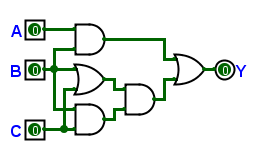
\includegraphics[width=\maxwidth{.95\linewidth}]{gfx/05_04}
	\caption{Example Circuit}
	\label{fig:05_04}
\end{figure}

To generate the Boolean equation for a circuit, write the output of each gate as determined by the input signals and type of gate, working from the inputs to the final output. Figure \ref{fig:05_05} illustrates the result of this process.

\begin{figure}[H]
	\centering
	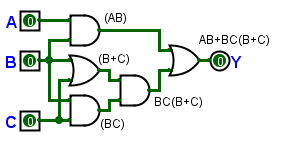
\includegraphics[width=\maxwidth{.95\linewidth}]{gfx/05_05}
	\caption{Example Circuit With Gate Outputs}
	\label{fig:05_05}
\end{figure}

This process leads to Equation \ref{05:eq:equation_from_circuit}.

\begin{align}
  \label{05:eq:equation_from_circuit}
  AB+BC(B+C) &= Y
\end{align}

\subsection{Starting From a Boolean Equation}
\label{05:subsec:starting_from_a_boolean_equation}

If a logic circuit's function is expressed as a Boolean equation, then algebraic methods can be applied to reduce the number of logic gates, resulting in a circuit that performs the same function with fewer components. As an example, Equation \ref{05:soln:equation_to_simplify_one_solution} simplifies the circuit found in Figure \ref{05:fig:circuit_with_boolean_expression}. 

\begin{align}
\label{05:soln:equation_to_simplify_one_solution}
  AB+BC(B+C) && \text{Original Expression} \\
  \nonumber
  AB+BBC+BCC && \text{Distribute BC} \\
  \nonumber
  AB+BC+BC && \text{Idempotence: BB=B and CC=C} \\
  \nonumber
  AB+BC && \text{Idempotence: BC+BC=BC} \\
  \nonumber
  B(A+C) && \text{Factor} 
\end{align}

The final expression, $ B(A + C) $, requires only two gates, and is much simpler than the original, yet performs the same function. Such component reduction results in higher operating speed (less gate propagation delay), less power consumption, less cost to manufacture, and greater reliability. 

As a second example, consider Equation \ref{05:eq:equation_to_simplify_two}.

\begin{align}
  \label{05:eq:equation_to_simplify_two}
  A+AB &= Y
\end{align}

This is simplified below.

\begin{align}
\label{05:soln:equation_to_simplify_two}
  A+AB && \text{Original Expression} \\
  \nonumber
  A(1+B) && \text{Factor} \\
  \nonumber
  A(1) && \text{Annihilation (1+B=1)} \\
  \nonumber
  A && \text{Identity A1=A}
\end{align}

The original expression, $ A+AB $ has been reduced to  $ A $ so the original circuit could be replaced by a wire directly from input  $ A $ to output  $ Y $. Equation \ref{05:eq:equation_to_simplify_three} looks similar to Equation \ref{05:eq:equation_to_simplify_two}, but is quite different and requires a more clever simplification.

\begin{align}
  \label{05:eq:equation_to_simplify_three}
  A+A'B &= Y
\end{align}

This is simplified below.

\begin{align}
  \label{05:soln:equation_to_simplify_three}
  A+A'B && \text{Original Expression} \\
  \nonumber
  A+AB+A'B && \text{Expand A to A+AB (Absorption)} \\
  \nonumber
  A+B(A+A') && \text{Factor B out of the last two terms} \\
  \nonumber
  A+B(1) && \text{Complement Property} \\
  \nonumber
  A+B && \text{Identityt: B(1)=B} 
\end{align}

Note how the Absorption Property ($ A + AB = A $) is used to ``un-simplify'' the first  $ A $ term, changing  $ A $ into $ A + AB $. While this may seem like a backward step, it ultimately helped to reduce the expression to something simpler. Sometimes ``backward'' steps must be taken to achieve the most elegant solution. Knowing when to take such a step is part of the art of algebra. 

As another example, simplify this \gls{pos} expression equation: 

\begin{align}
  \label{05:eq:equation_to_simplify_four}
  (A+B)(A+C) &= Y
\end{align}

This is simplified below.

\begin{align}
  \label{05:soln:equation_to_simplify_four}
  (A+B)(A+C) && \text{Original Expression} \\
  \nonumber
  AA+AC+AB+BC && \text{Distribute A+B} \\
  \nonumber
  A+AC+AB+BC && \text{Idempotence: AA=A} \\
  \nonumber
  A+AB+BC && \text{Absorption: A+AC=A} \\
  \nonumber
  A+BC && \text{Absorption: A+AB=A}
\end{align}

In each of the examples in this section, a Boolean expression was simplified using algebraic methods, which led to a reduction in the number of gates needed and made the final circuit more economical to construct and reliable to operate. 

\subsection{Practice Problems}
\label{05:subsec:practice_problems_for_simplifying_with_algebra}

Table \ref{05:tab:simplifying_boolean_expressions} shows a Boolean expression on the left and its simplified version on the right. This is provided for practice in simplifying expressions using algebraic methods. 

\begin{table}[H]
  \sffamily
  \newcommand{\head}[1]{\textcolor{white}{\textbf{#1}}}    
  \begin{center}
    \rowcolors{2}{gray!10}{white} % Color every other line a light gray
    \begin{tabular}{cc}
      \rowcolor{black!75}
      \head{Original Expression} & \head{Simplified} \\
      $ A(A'+B) $ & $ AB $ \\
      $ A+A'B $ & $ A+B $ \\
      $ (A+B)(A+B') $ & $ A $ \\
      $ AB+A'C+BC $ & $ AB+A'C $ \\
    \end{tabular}
  \end{center}
  \caption{Simplifying Boolean Expressions}
  \label{05:tab:simplifying_boolean_expressions}
\end{table}